%---------------------------------------------------------------
\chapter{SRAM PUF experiments and implementation on ESP32}\label{sec:implementation}
%---------------------------------------------------------------

% uvod s tim ze pouzivam esp32, cislovani, jake desky?, komoru, jake teploty?, nominal voltage...

The goal of this chapter is to find a suitable mechanism for \gls{sram} power state control on the ESP32 microcontroller. Two different methods are presented and their result (the startup memory values used as a \gls{puf} response) are analyzed. 

First, an analysis based on temperature and \gls{sram} power off-time is performed. The temperature is controlled by a temperature chamber Binder MK-56obj. It is capable of producing temperatures from -40~°C to +180~°C~\cite{Binder2021}. However, only the range of -40~°C to +70~°C is used for the analysis as higher temperatures could potentially damage the components. This analysis is performed mainly to understand the data retention time of the \gls{sram} and set an adequate minimum interval the memory needs to stay off before extracting the response.

Then, some of the \gls{puf} parameters defined in Section~\ref{sec:puf_evaluation} are used to evaluate the results. A summary of both power state control methods is provided at the end, discussing their advantages, disadvantages and viability of use.

Only the original ESP32 microcontroller model is used. Sixteen pieces will be measured and they are numbered from \gls{mcu} 1 to \gls{mcu} 16. All of the measurements were captured under normal voltage conditions. 

%--------------------------------
\section{RTC SRAM based PUF}
%--------------------------------

The first method of \gls{sram} power control is to use the \gls{rtc} part of \gls{sram} memory on ESP32. This part of memory can be switched on and off using the \gls{rtc} power domain controller.
 
\subsection{RTC SRAM power control}

The ESP32 has the ability to power-control parts of its chip. This feature can be used to save power while some of the components of the microcontroller are not being used. WiFi, digital core, internal \gls{sram} and \gls{rtc} \gls{sram} can all be power-controlled. This seems like an ideal mechanism for implementing the \gls{sram} \gls{puf} as the memory can be turned off and on during runtime with little time overhead.~\cite{esp322021}

All of the individual \gls{sram} sections (SRAM 0, 1 and 2, \gls{rtc} FAST \gls{sram} and \gls{rtc} SLOW \gls{sram}, described in more detail in Section~\ref{sec:memory_layout}) can be power-controlled individually. One of the sections, therefore, needs to be selected for the \gls{puf} implementation.

At first, the logical \gls{sram} section to select would be the \gls{sram} 0, 1 or 2, as they have a large capacity (all three more than 100 KB). However, all of the data saved in the selected section would be lost during response extraction (the memory needs to be turned off). This would prohibit this chunk of memory from being used and potentially render some memory-hungry applications impossible to be implemented. Additionally, the ESP-IDF toolchain would need to be adjusted to not use this part of memory. 

\begin{figure}[ht!]
    \centering
    \captionsetup{justification=centering,margin=0.5cm}
    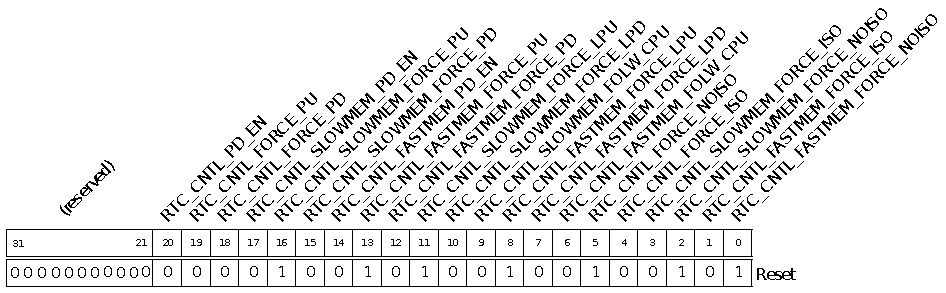
\includegraphics[width=\textwidth]{images/rtc_register.pdf}
    \caption[RTC domain power management register (address 0x3FF48080)]{RTC domain power management register (address 0x3FF48080)~\cite{esp322021}}
    \label{fig:rtc_register}
\end{figure}

Because of these drawbacks, the \gls{rtc} FAST \gls{sram} section was selected. Since it is also used to store program instructions (the deep sleep wake stub) and data (dynamic heap allocations), it needs to be preserved during response extraction. This can be done by backing up the whole 8 KB section of memory to the main \gls{sram} before powering down and restoring it afterwards. This is not possible with the main \gls{sram} sections because of their size.

The power state of the FAST \gls{rtc} \gls{sram} is controlled by the \gls{rtc} domain power management register. Functions of the individual register bits are shown in Figure~\ref{fig:rtc_register}. Bits number 13 (\lstinline{RTC_CNTL_FASTMEM_FORCE_PU}\footnote{\lstinline{RTC_CNTL_FASTMEM_FORCE_PD} = \gls{rtc} control fast memory force power up}) and 12 (\lstinline{RTC_CNTL_FASTMEM_FORCE_PD}\footnote{\lstinline{RTC_CNTL_FASTMEM_FORCE_PD} = \gls{rtc} control fast memory force power down}) are important. They can be set to control the power state of the memory.~\cite{esp322021}

\subsection{SRAM analysis based on temperature and power-off time}\label{sec:rtc_analysis}

Data remanence of the \gls{rtc} FAST \gls{sram}, power controlled using the above-described method, is analyzed in this section. Several experiments for each \gls{mcu} have been conducted according to this algorithm:

\begin{enumerate}
    \item Set the ambient temperature to the desired value.
    \item Initialize memory to a default value.\footnote{In the presented experiments, the default value was `0' for all bits. However, measurements with bits initialized to `1' showed nearly identical results.}
    \item Turn memory off for a set interval and then turned it on again.
    \item Observe the contents of memory.
    \item Continue from step 2. with an increased turn off interval until enough data is collected.
\end{enumerate}

Observing the contents of memory, in this case, means calculating the percentage of bits that flipped to a different state while turned off. For the default initial state of `0', this is equivalent to calculating the percentage Hamming weight of the bit string (counting the `1' bits).

The expected result is that, at the beginning for a very small turn off interval, no bits will flip. The biggest interval under which no bits flip is the \emph{data remanence time}. With increasing turn off interval, more and more bits start to flip. The percentage of flipped bits should stabilize around 50\% which is the ideal value of uniformity. At this point, all data previously saved in memory should be lost and the contents of memory after power up should depend only on the preferred initial state of the memory cells. The smallest interval under which this happens will be called the \emph{fade-out time}. The \gls{sram} \gls{puf} implementation should set the turn off interval to a greater value than the maximum \emph{fade-out time} of the \gls{sram} under varying conditions (such as temperature or voltage). This prevents data remanence from affecting the \gls{puf} response.

The results of the first experiment are displayed in Figure~\ref{fig:all_plus_20_rtc}. The graph shows the percentage of flipped bits at 20 °C with the turn off interval ranging from 0 to 1000 $\mu{}S$. The results are as expected. The \emph{data remanence time} is around 180 $\mu{}S$, the \emph{fade-out time} is around 900 $\mu{}S$ and the percentage of flipped bits stabilizes around 50\% for all \glspl{mcu}.

\begin{figure}[ht!]
    \centering
    \captionsetup{justification=centering,margin=0.5cm}
    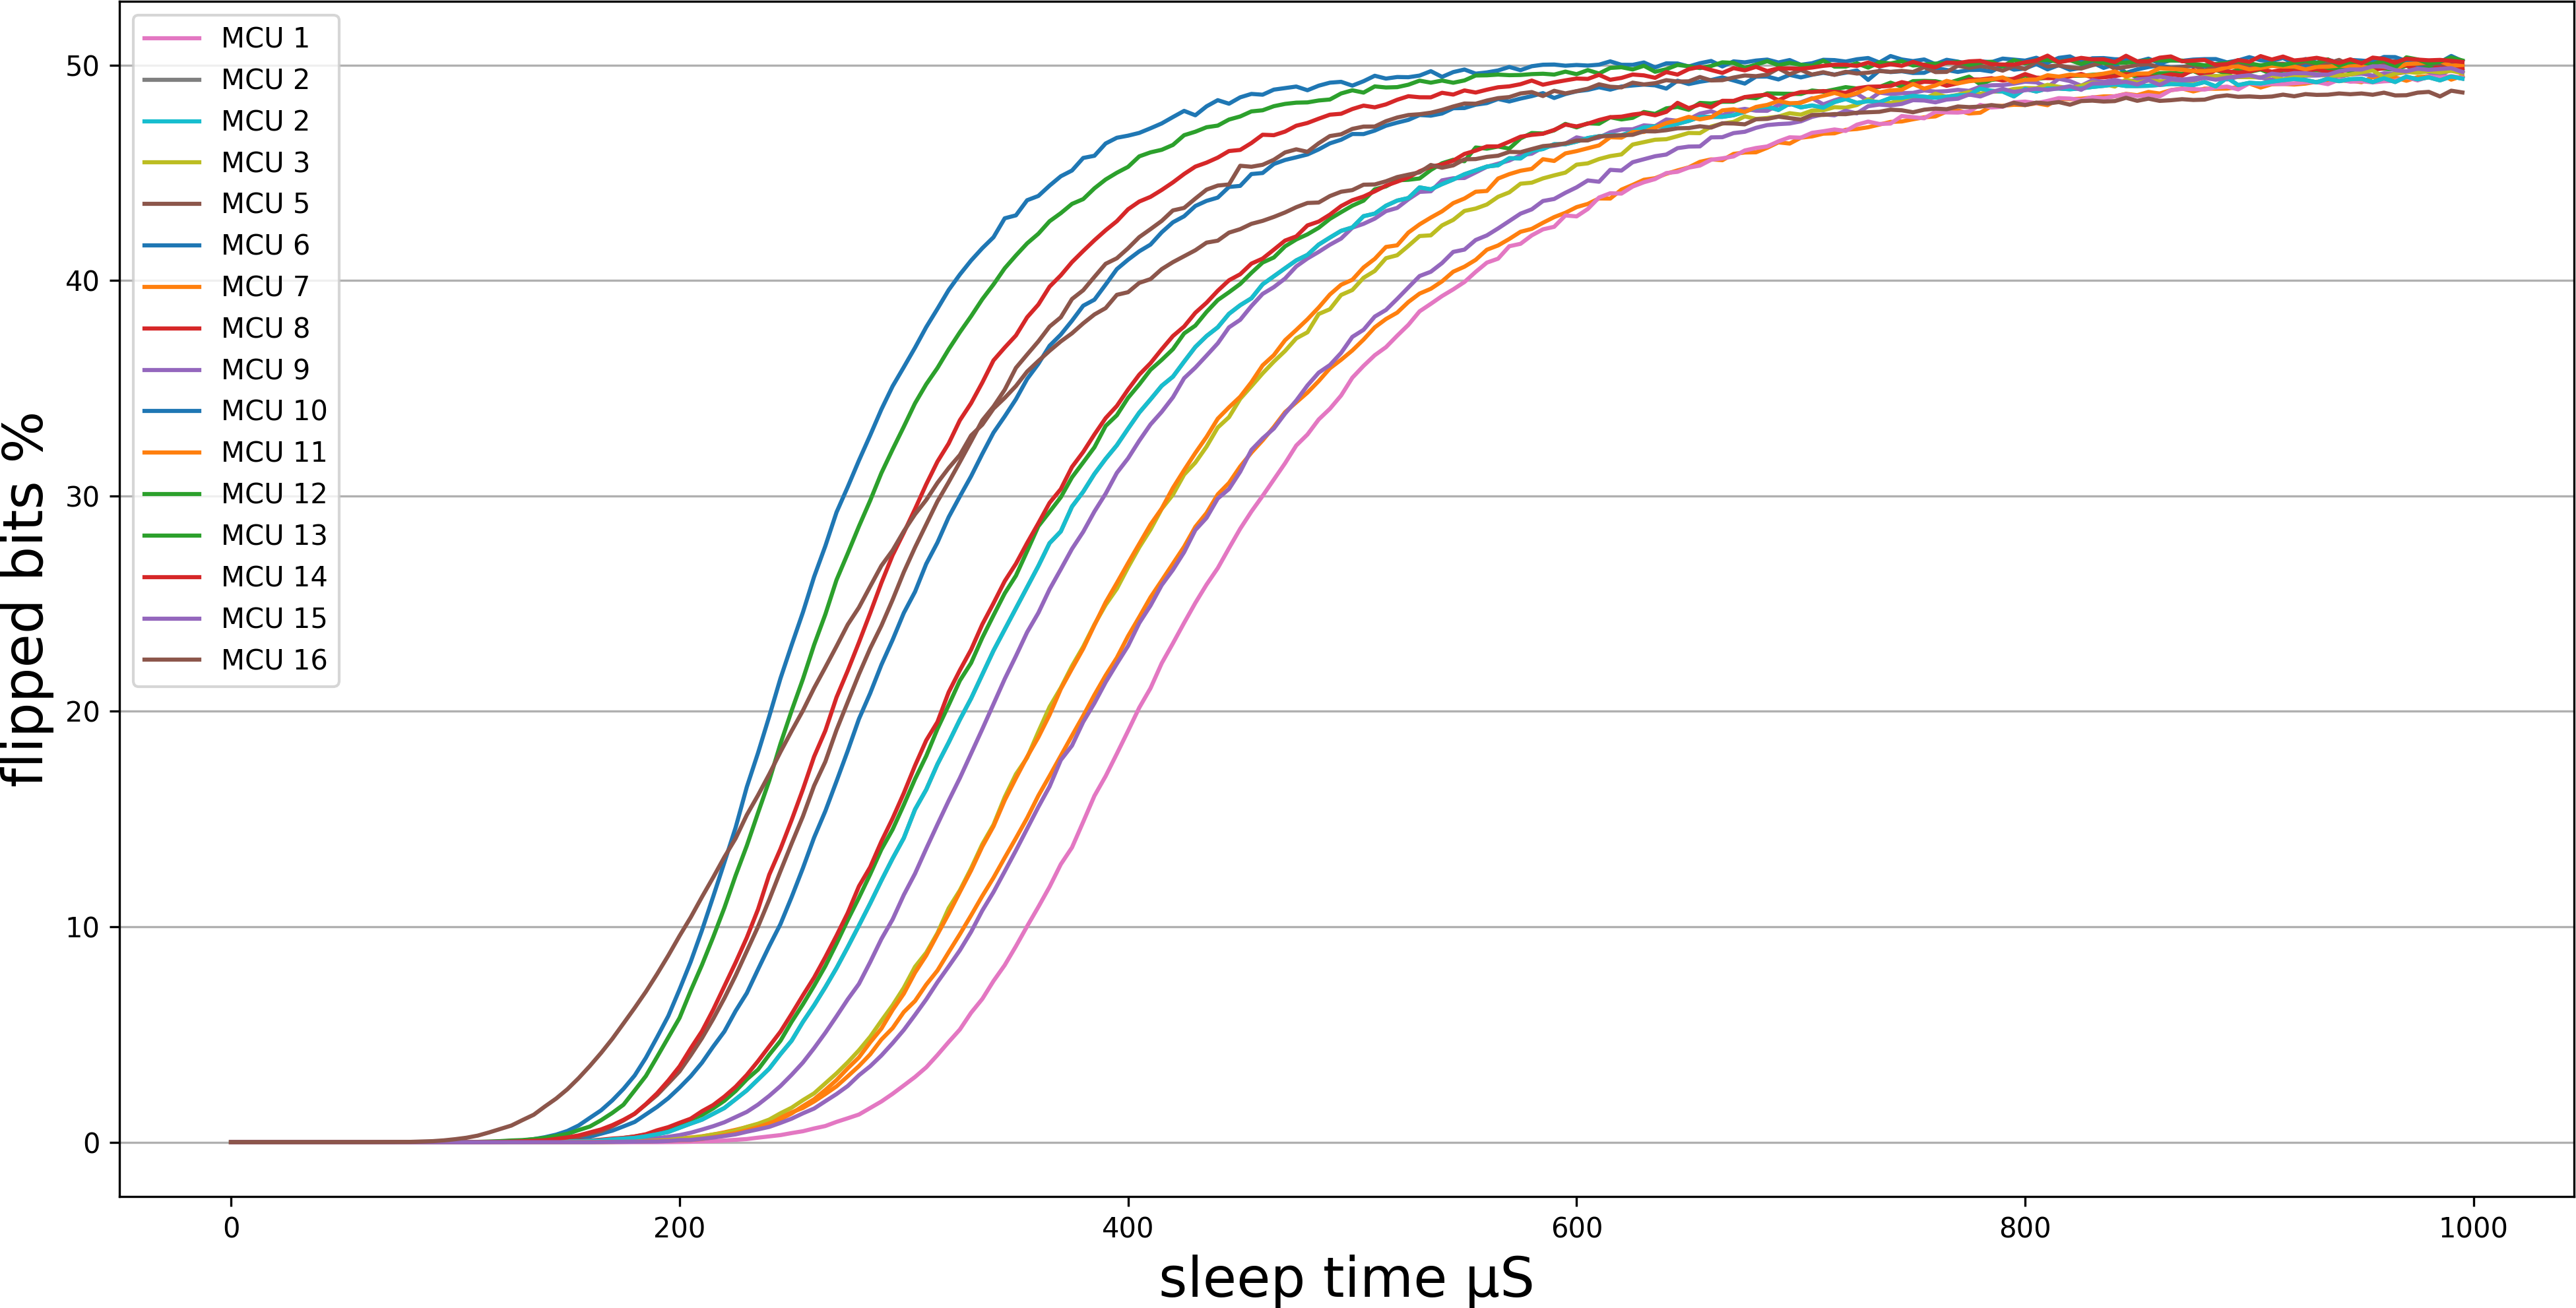
\includegraphics[width=\textwidth]{images/all_plus_20_rtc.png}
    \caption{Percentage of flipped bits of all MCUs at 20 °C (RTC SRAM method)}
    \label{fig:all_plus_20_rtc}
\end{figure}


The second experiment shows the behavior of one \gls{mcu} (number 6 was chosen but results for the others are similar) across the whole range of -40 to +70 °C. The graph can be seen in Figure~\ref{fig:6_across_temps_rtc}. As expected, the lower temperatures increase the \emph{data remanence time} and the \emph{fade-out time} significantly and higher temperatures decrease them. However, for the lower temperatures (below 0 °C), the \emph{fade-out time} cannot be seen as the memory did not have enough time to stabilize yet. 

\begin{figure}[ht!]
    \centering
    \captionsetup{justification=centering,margin=0.5cm}
    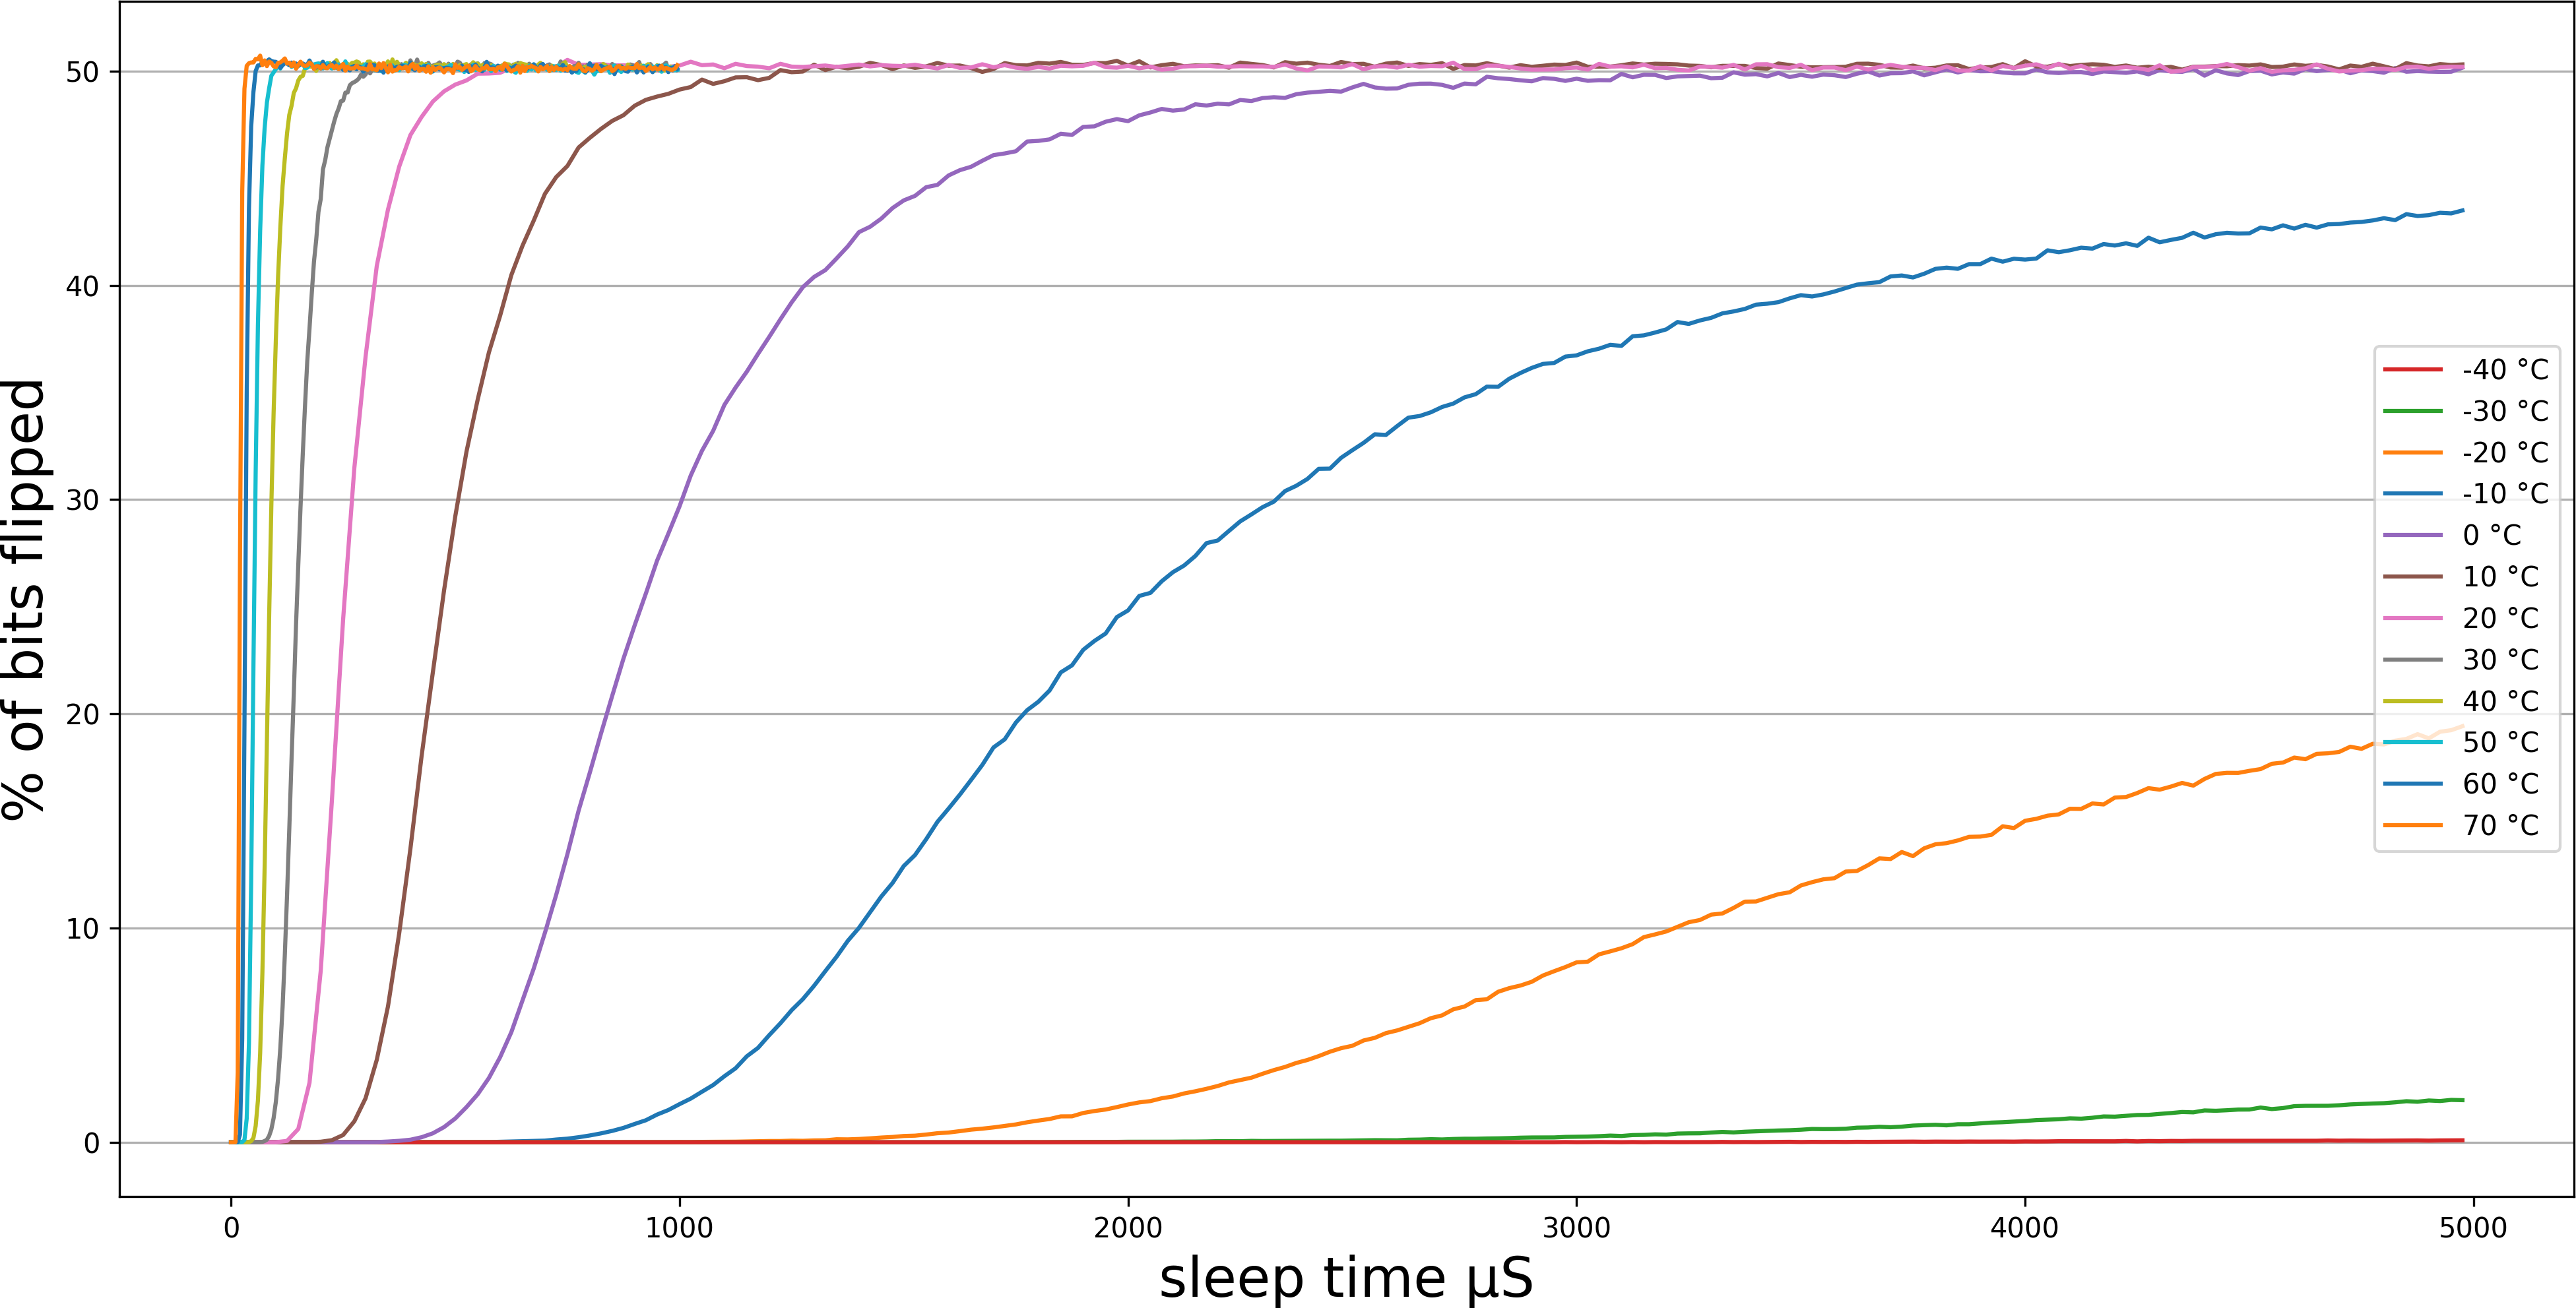
\includegraphics[width=\textwidth]{images/6_across_temps_rtc.png}
    \caption{Percentage of flipped bits of MCU 6 across a range of temperatures (RTC SRAM method)}
    \label{fig:6_across_temps_rtc}
\end{figure}

The next experiment, therefore, looks at the behavior of all \glspl{mcu} at -20~°C. The turn off interval was significantly increased to 50 000~$\mu{}S$. The results are displayed in Figure~\ref{fig:all_minus_20_rtc}. A very strange behavior can be seen. It looks as if the memory does not fade-out at all, only a limited number of bits flip and the rest of the bits retain their original state. Furthermore, for each board, a wildly different number of bits flip in this temperature. Nearly no bits flip for \gls{mcu} 4, but about 33 percent of bits flip for \gls{mcu} 6.\footnote{Note the values on the Y-axis of the graph, they do not even reach 50~\%.}

This was confirmed by extending the range of the turn off interval to 1 S and then to 100 S. The number of flipped bits does not change anymore with increased turn off time and the memory `freezes'. At -40~°C only about 1 \% of bits flip no matter the turn off interval for each \gls{mcu}. The initial value of the memory cell does not matter either, `0' and `1' states both freeze in the same way. 

\begin{figure}[ht!]
    \centering
    \captionsetup{justification=centering,margin=0.5cm}
    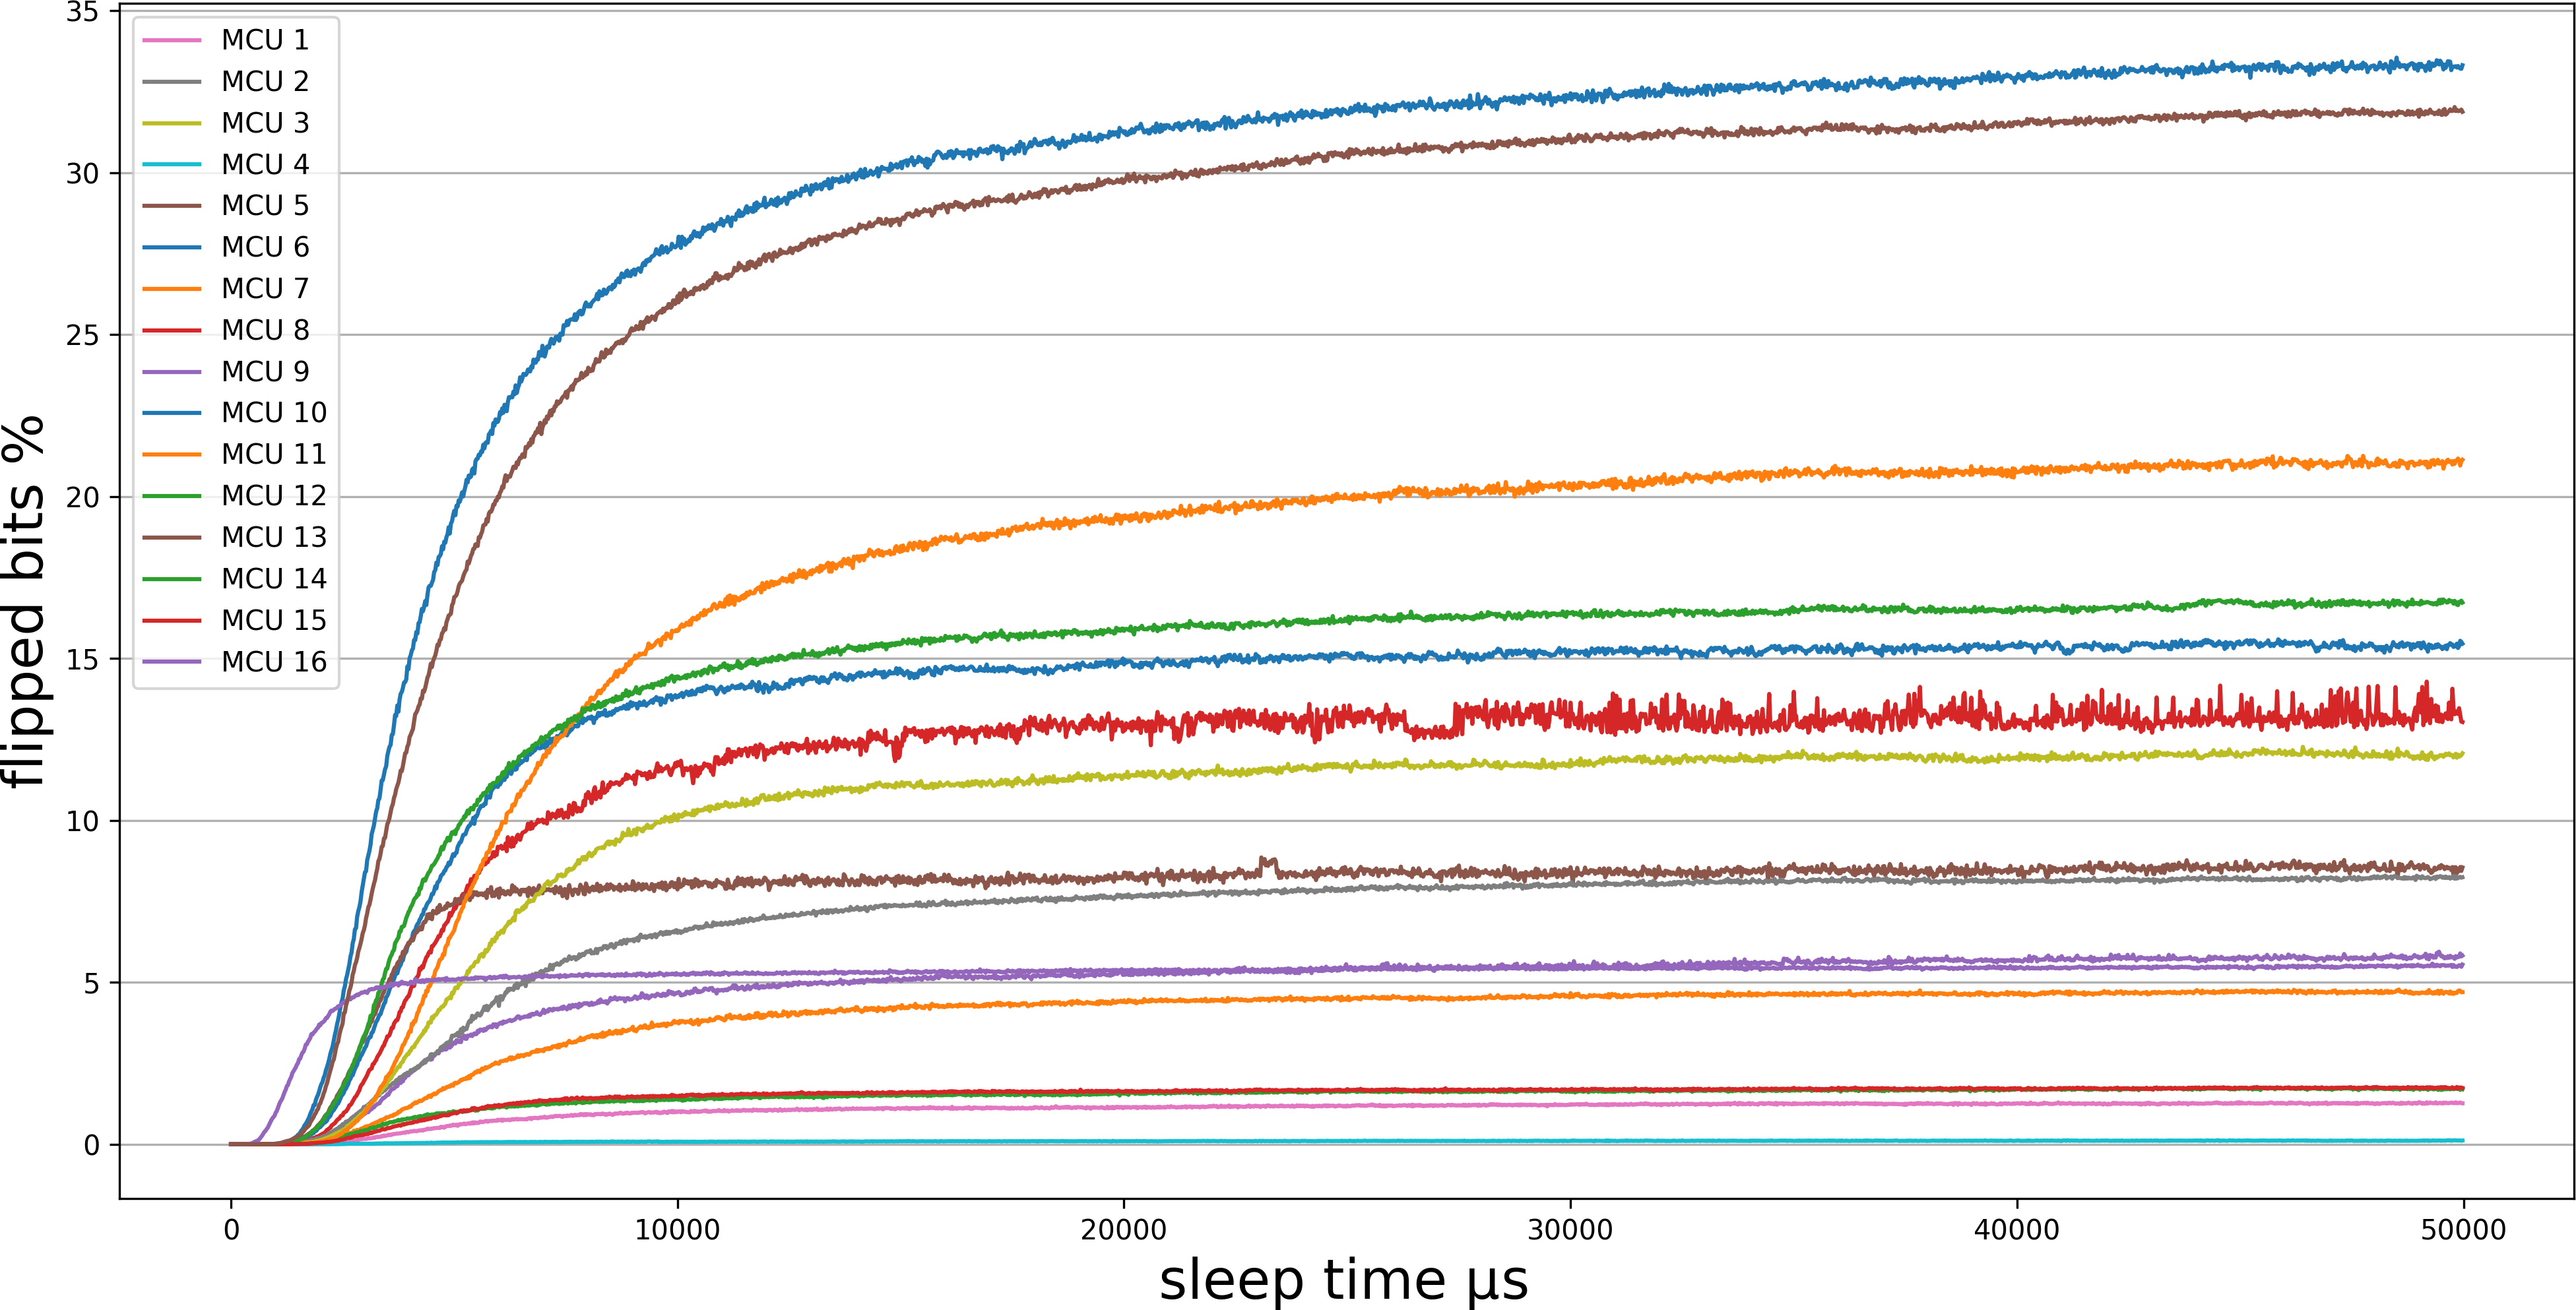
\includegraphics[width=\textwidth]{images/all_minus_20_rtc.png}
    \caption{Percentage of flipped bits of all MCUs at -20 °C (RTC SRAM method)}
    \label{fig:all_minus_20_rtc}
\end{figure}

A possible explanation of this behavior can be the following. All transistors leak current even if they are switched off. This is called a leakage current. A transistor that works as a switch for turning the \gls{rtc} FAST \gls{sram} on and off has a leakage current that is high enough that the memory is able to retain its state in low temperatures. \gls{sram} memory draws very little power while only retaining data---no read/write operations are taking place and thus the logical states of the circuit do not change. This is called static \gls{cmos} power dissipation. It has been shown by~\cite{Kocanda2015} that the static power dissipation is highly influenced by temperature. A change of temperature from 100 to 20~°C decreases the power draw by a factor of 3 to 83, depending on the exact \gls{cmos} technology used.

As is evident from the Figure~\ref{fig:all_minus_20_rtc}, different \glspl{mcu} freeze at different rates---the percentage of bit flips varies wildly across \glspl{mcu}. This supports this hypothesis as the leakage current of the transistor is probably also influenced by the random variations during the manufacturing process.

This can explain the `freezing' effect of memory in low temperatures. However, this explanation could not be confirmed.

\subsection{PUF evaluation parameters}\label{sec:rtc_evaluation}

Since the evaluation parameters require \gls{puf} responses for their calculation, they need to be obtained. The response was chosen to be a 4~KB bit string of the (first half of) \gls{rtc} FAST \gls{sram}. Only one response is extracted, no memory address based challenge system was considered because of the limited size of the used memory region (8 KB). The turn off interval was set to 10 000~$\mu{}S$. This is a lot higher value than the \emph{fade-out time} of the memory for warmer temperatures (above 0~°C). There is no point in considering lower temperatures since the memory freezes while using this power control technique. The reference response was calculated using a bitwise average of 1000 measured responses.

\subsubsection*{Uniformity}

Uniformity of all \glspl{mcu} in different temperatures can be seen in Table~\ref{table:uniformity_rtc_sram}. The values look very good at temperatures above 10~°C, hovering around the desired value of 50~\%. However, in lower temperatures, the effect of memory freezing can be seen clearly. The values plummet and hit nearly 0~\% at -40~°C. This is due to the choice of default initial value of `0' bits. Uniformity rises towards 100~\% if the default value is a `1' bit.

\begin{table}[ht!]
    \centering
    \begin{tabular}{c||rrrrrrrrrr}
\toprule
\textbf{MCU} & \textbf{-40°C} & \textbf{-30°C} & \textbf{-20°C} & \textbf{-10°C} & \textbf{0°C} & \textbf{10°C} & \textbf{20°C} & \textbf{30°C} & \textbf{50°C} & \textbf{70°C} \\
\midrule
1    &   0.00 &   0.06 &   1.26 &  10.27 & 38.00 & 48.94 & 49.93 & 49.89 & 49.92 & 49.91 \\
2    &   0.05 &   0.55 &   8.32 &  25.05 & 44.08 & 49.29 & 49.52 & 49.65 & 49.81 & 49.88 \\
3    &   0.23 &   1.88 &  12.06 &  34.63 & 46.89 & 49.76 & 49.92 & 49.91 & 49.98 & 49.99 \\
4    &   0.00 &   0.00 &   0.10 &   2.74 & 14.74 & 41.72 & 49.95 & 50.18 & 50.36 & 50.38 \\
5    &   0.16 &   1.85 &   8.09 &  27.40 & 44.46 & 49.96 & 50.02 & 50.06 & 50.11 & 50.12 \\
6    &   1.11 &  10.82 &  33.17 &  47.60 & 50.11 & 50.18 & 50.09 & 50.08 & 50.06 & 50.04 \\
7    &   0.45 &   7.71 &  21.45 &  39.26 & 49.45 & 50.11 & 50.17 & 50.20 & 50.29 & 50.29 \\
8    &   0.18 &   2.41 &  14.03 &  25.69 & 45.20 & 49.96 & 49.84 & 49.92 & 49.98 & 50.00 \\
9    &   0.07 &   0.57 &   5.69 &  20.71 & 39.98 & 49.14 & 49.76 & 49.79 & 49.78 & 49.82 \\
10   &   0.17 &   2.91 &  15.35 &  37.38 & 48.65 & 49.83 & 49.96 & 49.99 & 50.03 & 50.04 \\
11   &   0.05 &   0.40 &   4.75 &  23.70 & 43.60 & 49.88 & 50.24 & 50.18 & 50.26 & 50.31 \\
12   &   0.00 &   0.07 &   1.63 &  16.19 & 38.21 & 48.25 & 49.96 & 49.96 & 49.89 & 49.86 \\
13   &   0.80 &  12.58 &  31.70 &  44.66 & 49.76 & 49.98 & 50.08 & 50.10 & 50.07 & 50.01 \\
14   &   0.18 &   2.44 &  16.75 &  39.50 & 49.43 & 50.09 & 50.16 & 50.19 & 50.14 & 50.17 \\
15   &   0.01 &   0.11 &   1.74 &  17.96 & 36.05 & 48.30 & 50.13 & 50.18 & 50.17 & 50.13 \\
16   &   0.77 &   2.02 &   5.48 &  13.92 & 30.52 & 44.13 & 49.55 & 49.74 & 49.81 & 49.90 \\
\textbf{mean} &   0.27 &   2.90 &  11.35 &  26.67 & 41.82 & 48.72 & 49.96 & 50.00 & 50.04 & 50.05 \\
\bottomrule
\end{tabular}
    \captionsetup{justification=centering,margin=0.5cm}
    \caption{Uniformity (\%) across all MCUs and temperatures (RTC SRAM method, 10 mS turn off interval)}
    \label{table:uniformity_rtc_sram}
\end{table}

\subsubsection*{Reliability}

Reliability values of all \glspl{mcu} in different temperatures are displayed in Table~\ref{table:reliability_rtc_sram}. The reference response used for the calculations was obtained at 20~°C.

Once again, the values look good in temperatures above 10 °C, being fairly close to the ideal 100~\%. The highest reliability can be observed at 20~°C. This is the result of the reference response being calculated at this temperature. The effect of freezing is once again evident in low temperatures. Reliability goes down toward 50~\%, which is the worst possible value.\footnote{The value of 0~\% would mean that the response bits are just inverted compared to the reference.} 

\begin{table}[ht!]
    \centering
    \begin{tabular}{c||rrrrrrrrrr}
    \toprule
    \textbf{MCU} & \textbf{-40°C} & \textbf{-30°C} & \textbf{-20°C} & \textbf{-10°C} & \textbf{0°C} & \textbf{10°C} & \textbf{20°C} & \textbf{30°C} & \textbf{50°C} & \textbf{70°C} \\
    \midrule
    1    &  50.16 &  52.80 &  63.34 &  80.56 & 87.36 & 93.70 & 96.55 & 95.41 & 93.96 & 93.25 \\
    2    &  49.71 &  50.06 &  54.19 &  71.71 & 88.36 & 94.19 & 97.35 & 95.71 & 93.72 & 93.06 \\
    3    &  50.04 &  50.10 &  51.61 &  65.27 & 84.11 & 89.41 & 96.99 & 93.54 & 90.39 & 89.82 \\
    4    &  50.46 &  52.60 &  62.97 &  71.01 & 81.68 & 91.70 & 96.65 & 95.61 & 94.22 & 93.65 \\
    5    &  50.33 &  50.82 &  55.72 &  68.29 & 80.18 & 90.17 & 96.75 & 94.94 & 93.05 & 92.53 \\
    6    &  50.20 &  51.86 &  57.55 &  71.77 & 81.84 & 93.09 & 96.63 & 95.67 & 94.48 & 93.81 \\
    7    &  50.08 &  50.13 &  51.27 &  59.75 & 82.78 & 90.01 & 96.86 & 94.07 & 89.99 & 88.93 \\
    8    &  50.56 &  51.04 &  58.27 &  72.19 & 83.89 & 92.07 & 96.70 & 94.55 & 91.32 & 90.30 \\
    9    &  50.29 &  51.91 &  60.69 &  79.92 & 87.22 & 93.40 & 96.75 & 95.59 & 93.94 & 93.16 \\
    10   &  50.09 &  50.09 &  50.19 &  52.76 & 64.25 & 88.26 & 97.45 & 93.60 & 88.17 & 86.39 \\
    11   &  50.91 &  59.56 &  77.59 &  86.35 & 91.16 & 94.87 & 96.38 & 95.92 & 95.14 & 94.30 \\
    12   &  50.31 &  57.04 &  68.94 &  78.72 & 86.82 & 93.98 & 96.53 & 95.81 & 94.73 & 94.08 \\
    13   &  50.69 &  61.81 &  77.67 &  81.53 & 87.42 & 95.28 & 96.65 & 96.06 & 95.22 & 94.47 \\
    14   &  50.00 &  52.19 &  65.25 &  82.92 & 89.61 & 94.80 & 96.61 & 95.70 & 94.50 & 93.70 \\
    15   &  49.89 &  49.99 &  51.60 &  66.71 & 82.06 & 89.75 & 96.94 & 93.16 & 89.77 & 89.06 \\
    16   &  51.17 &  52.33 &  55.64 &  63.53 & 78.56 & 90.84 & 98.31 & 92.24 & 80.72 & 76.13 \\
    \textbf{mean} &  50.31 &  52.77 &  60.15 &  72.06 & 83.58 & 92.22 & 96.88 & 94.85 & 92.08 & 91.04 \\
    \bottomrule
    \end{tabular}
    \captionsetup{justification=centering,margin=0.5cm}
    \caption{Reliability (\%) across all MCUs and temperatures (RTC SRAM method, 10~mS turn off interval)}
    \label{table:reliability_rtc_sram}
\end{table}

\subsubsection*{Uniqueness}

Uniqueness of the responses from different \glspl{mcu} across the whole range of temperatures is shown in Table~\ref{table:uniqueness_rtc_sram}. Again, the values look good in temperatures above 0 °C, attacking the ideal of 50 \%. However, in lower temperatures uniqueness plummets rapidly as the responses start to freeze. Since the initial value of memory is the same across the \glspl{mcu}, the data remanence kicks in and the responses start to become more and more alike.

\begin{table}[ht!]
    \centering
    \begin{tabular}{cc}
    \textbf{Temperature °C} & \textbf{Uniqueness \%} \\
    \toprule
    -40  &  0.53 \\
    -30  &  5.63 \\
    -20  & 20.18 \\
    -10  & 39.19 \\
    0    & 48.64 \\
    10   & 49.81 \\
    20   & 49.73 \\
    30   & 49.66 \\
    40   & 49.60 \\
    50   & 49.55 \\
    60   & 49.54 \\
    70   & 49.54 \\
    \textbf{mean} & 38.47 \\
    \bottomrule
    \end{tabular}
    \captionsetup{justification=centering,margin=0.5cm}
    \caption{Uniqueness (\%) across all MCUs and temperatures (RTC SRAM method, 10~mS turn off interval)}
    \label{table:uniqueness_rtc_sram}
\end{table}

\subsection{Summary}
% ze tohle jde jen na puvodnim ESP32 a single coru, protoze ostatni maji jiny rezim
As is evident from the experiments, this power control method can only be used at temperatures above 10~°C. The exact temperature where the memory starts to freeze also differs for each \gls{mcu}.

Moreover, only the original ESP32 and the ESP32-S2 (the single-core version) microcontrollers have the functionality to power-control the memory sections. In the newer models, this functionality was replaced by the `retention' mode of memory. This mode enables the memory to retain its data while no read/write operations need to take place, saving power in the process.~\cite{esp322021} Thus, this method cannot be applied to the newer models. Additionally, only 8 KB of memory is available. Though this is enough if the \gls{puf} is used for key generation, as will become evident in Chapter~\ref{sec:response_extraction}.

On the other side, the ability to power-control the memory during runtime is very powerful. The response can be extracted on demand quickly because the whole device does not need to be powered down and then up which is an extremely time-consuming process.

%--------------------------------
\section{Deep sleep based PUF}
%--------------------------------

The second method of \gls{sram} power control is to use the internal \gls{sram} memory on ESP32. This part of memory can be switched on and off using the deep sleep mode.

\subsection{Deep sleep SRAM power control}

During the deep sleep power-saving mode, most of the chip is powered down. The \glspl{cpu}, most of \gls{sram} and all digital peripherals are turned off. Only the \gls{rtc} controller, the \gls{ulp} coprocessor and the FAST and SLOW \gls{rtc} \gls{sram} remain powered on. 

Several sources can be used to wake the device up from deep sleep. The \gls{rtc} timer, external \gls{gpio}, touch sensor and the \gls{ulp} coprocessor can all be used for this purpose. Since most of the device was turned off, the whole booting process (described in Section~\ref{sec:device_startup}) must take place during wakeup.

The \gls{rtc} timer is the wake-up mechanism that was chosen for the \gls{sram} power control, as it enables setting a precise power off interval. However, the \gls{rtc} timer uses an internal 150kHz RC oscillator as its clock source. The exact oscillator frequency is affected by temperature. This results in a time drift for different operating temperatures. Fortunately, this should not affect the \gls{puf} implementation. The same time drift will occur both in the real response extraction and during experiments. Only the power off timing information has reduced accuracy. This was not an issue while using the \gls{rtc} \gls{sram} based power control method, since the \gls{cpu} (which performed the timing) is clocked using  a 480 Mhz \gls{pll} clock.~\cite{esp322021},~\cite{espidf2022}

Care needs to be taken while extracting the startup memory values. As the boot process of the device is fairly complex, it is difficult to know exactly what regions of memory stay uninitialized and what regions are used by the bootloaders or the FreeRTOS before our code is executed. Even if such an uninitialized region of memory was found, it is not guaranteed that it will stay this way after a software update. The linker can assign new variables to this memory region or the old variables might be reordered. The memory would then be set to program data before we could extract the startup values.

To prevent this from happening, a process for extracting the startup values early in device boot was designed using the \emph{deep sleep wake stub}:

\begin{enumerate}
    \item After wakeup, the first stage bootloader calls the custom \emph{deep sleep wake stub} function
    \item The \emph{deep sleep wake stub} runs before the majority of other boot code. Therefore, it sees nearly the whole \gls{sram} memory uninitialized. A 4 KB of data from address 0x3FFB0000 is copied to a statically allocated buffer.
    \item The rest of the boot process continues.
    \item After boot, the startup data is found untouched in the buffer.
\end{enumerate}

The 0x3FFB0000 address (which is an address into the internal \gls{sram} 2) was chosen arbitrarily. Any address of the internal \gls{sram} 0, 1 or 2 can be chosen except for their first few KB---they are used by the first-stage bootloader before the \emph{deep sleep wake stub} runs.

The statically allocated buffer is not overwritten during the boot process because it is annotated by a \emph{NOINIT\_ATTR} attribute in the source code and is put into the \emph{no-init} section by the linker. This section is not initialized and was created to keep data during software resets.~\cite{espidf2022}

Copying the data to this buffer by the \emph{deep sleep wake stub} is necessary as the \emph{no-init} section can be moved by the linker to a different memory address. This could be prevented by altering the linker script in the ESP-IDF source. Though this would make the deployment of the resulting \gls{puf} implementation significantly more difficult.


\subsection{SRAM analysis based on temperature and power-off time}\label{sec:deep_sleep_analysis}

All of the experiments shown in this section were conducted using the same method that was explained at the beginning of Section~\ref{sec:rtc_analysis}. The above-described deep sleep power-control mechanism was used and the number of bit flips was calculated from 4~KB memory samples.

The first experiment shows the percentage of flipped bits across all \glspl{mcu} at -40~°C. The lowest temperature is shown as it is the most indicative of what value to choose for the turn off interval. The resulting graph can be seen in Figure~\ref{fig:all_minus_40_deep_sleep}. The \emph{data remanence time} for the \glspl{mcu} is approximately 1~200~$\mu{}S$ (this is more evident if the graph is zoomed in) and the \emph{fade-out time} is around 50~000~$\mu{}S$.

The effect of memory freezing in low temperatures is not present while using the deep sleep power-control method, as all the \glspl{mcu} stabilize around 50 \% of flipped bits.

\begin{figure}[ht!]
    \centering
    \captionsetup{justification=centering,margin=0.5cm}
    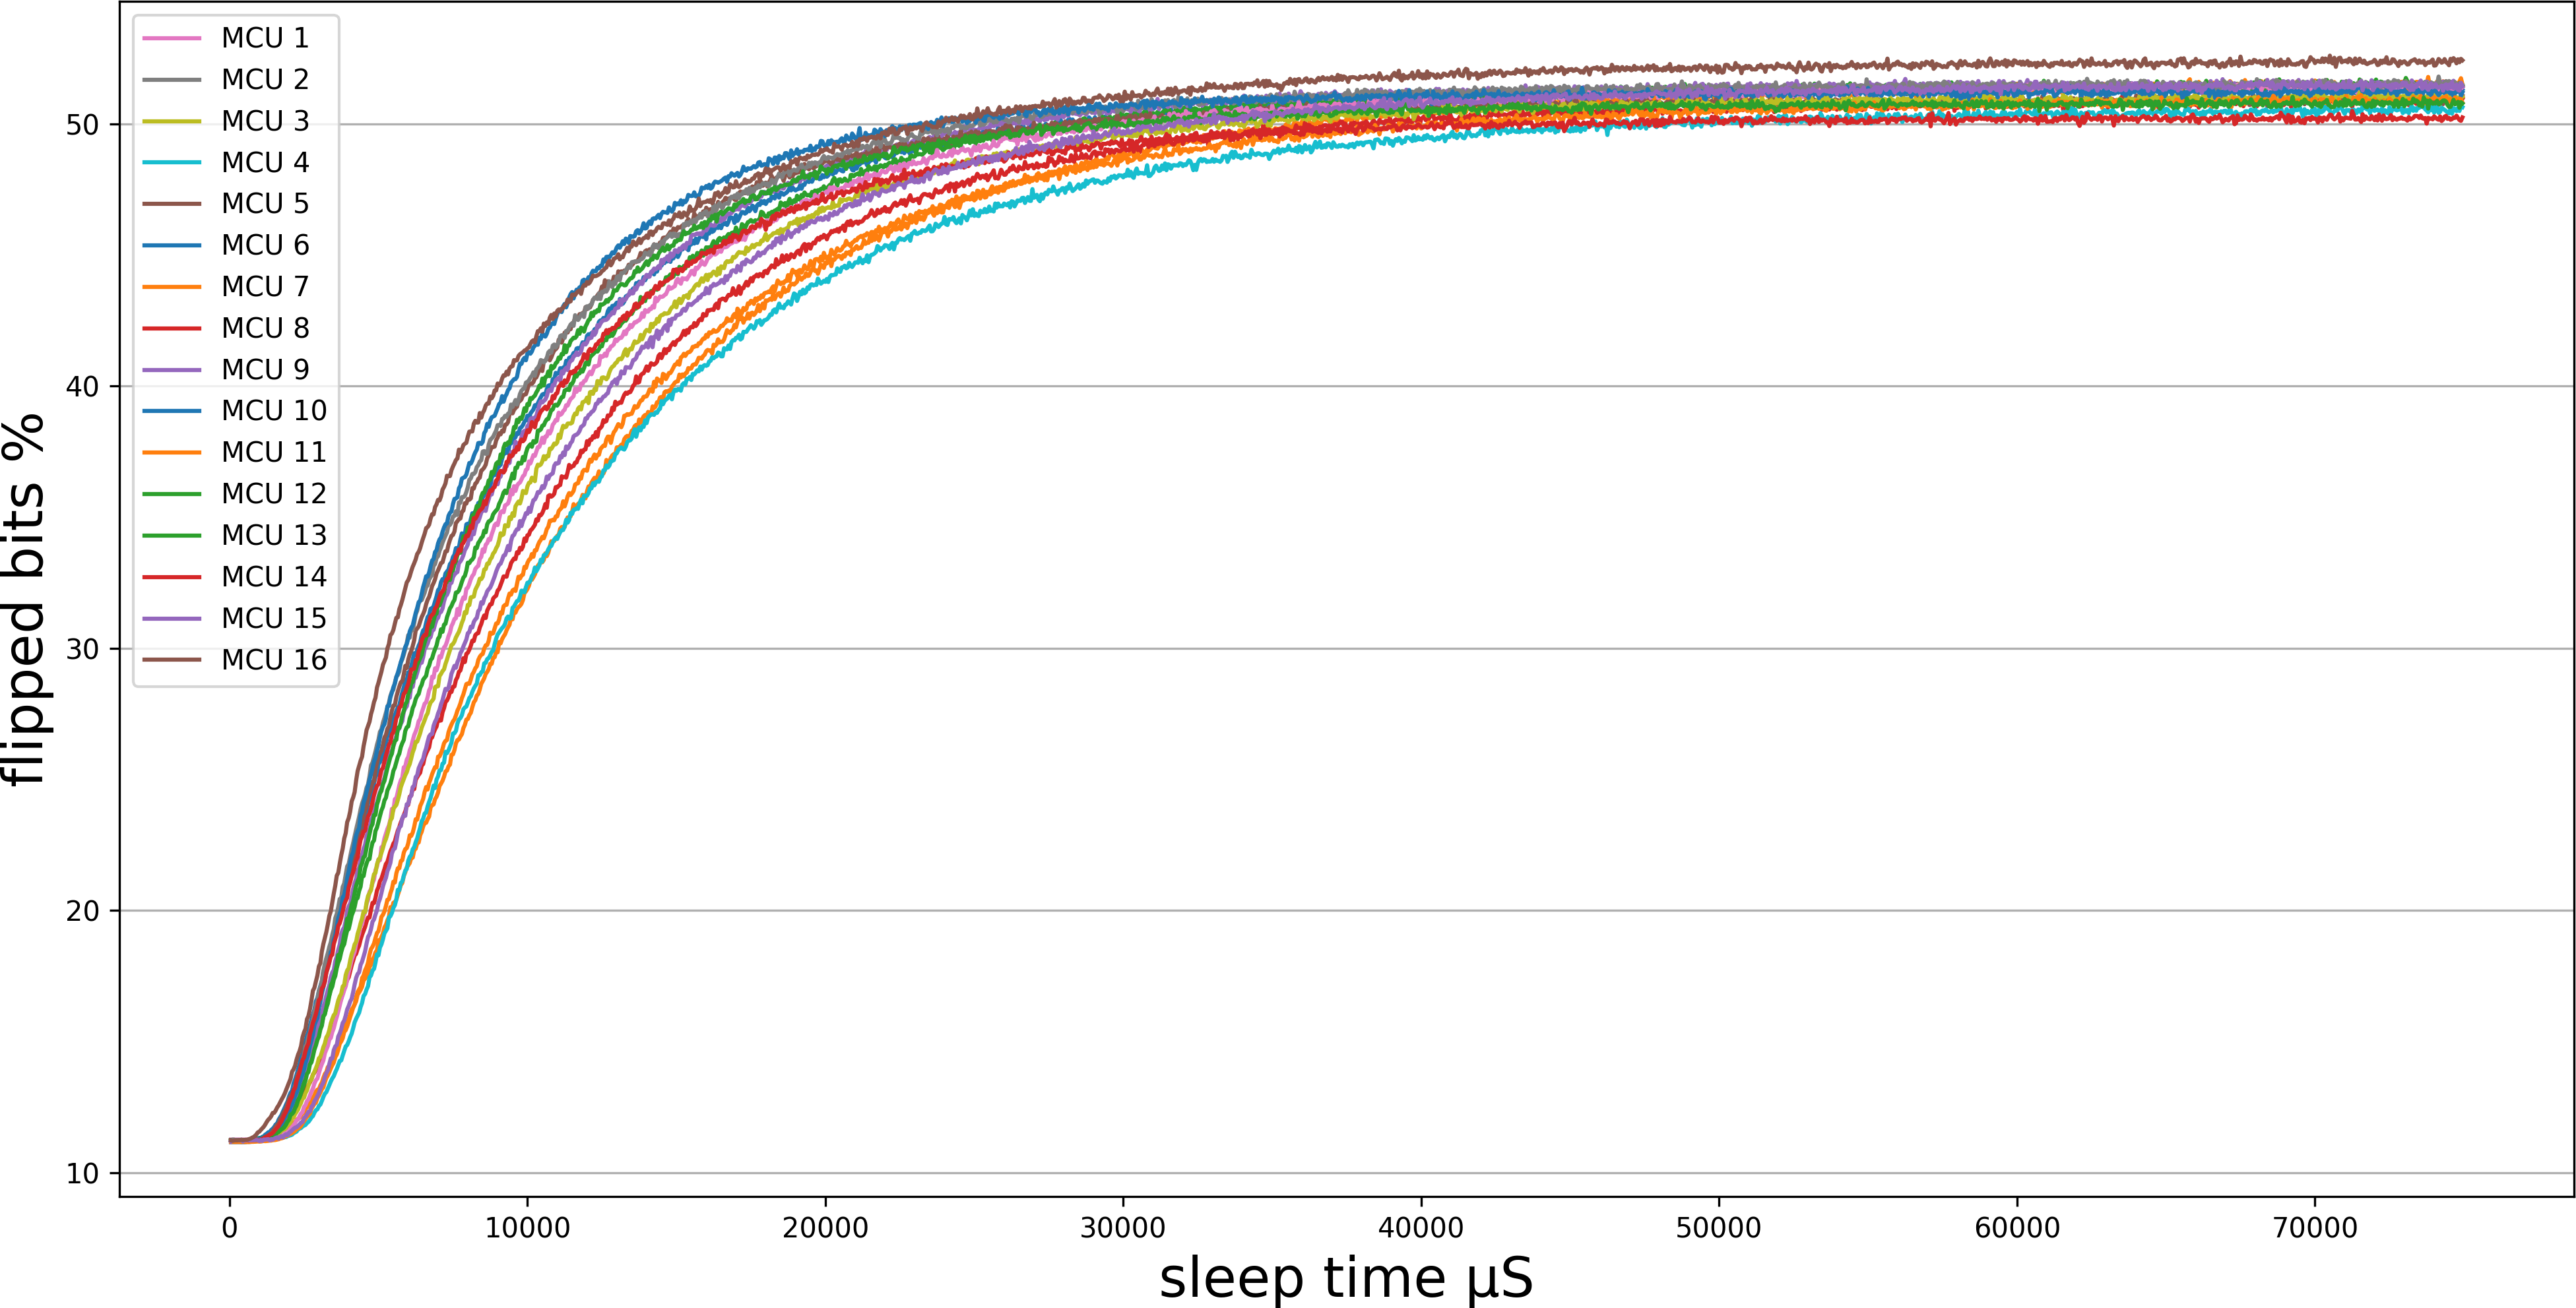
\includegraphics[width=\textwidth]{images/all_minus_40_deep_sleep.png}
    \caption{Percentage of flipped bits of all MCUs at -40 °C (deep sleep method)}
    \label{fig:all_minus_40_deep_sleep}
\end{figure}

The second experiment looks at the behavior of one \gls{mcu} (again, the number 6 was chosen but results for the others are similar) across the whole range of -40 to +70 °C. The results are shown in Figure~\ref{fig:6_across_temps_deep_sleep}. This time, since no memory freezing effect is present, the memory stabilizes around the value of 50 \% of flipped bits for all temperatures. It is also evident that the \emph{fade-out time} and the \emph{data remanence time} increase significantly with decreasing temperatures.

Note the data points for temperatures above 0~°C. Unexpectedly, they show a significant number of bit flips for very small turn off intervals (even for 0~$\mu{}S$). This behavior is caused by the \gls{rtc} controller that wakes up the chip from deep sleep. Even if the sleep time is set to 0~$\mu{}S$, the whole chip is put into deep sleep for at least 1~000~$\mu{}S$. This is probably caused by the design of the \gls{rtc} controller or the internal ESP-IDF software components. However, the deep sleep mode behaves as expected if the turn off interval is greater than 1~000~$\mu{}S$.

\begin{figure}[ht!]
    \centering
    \captionsetup{justification=centering,margin=0.5cm}
    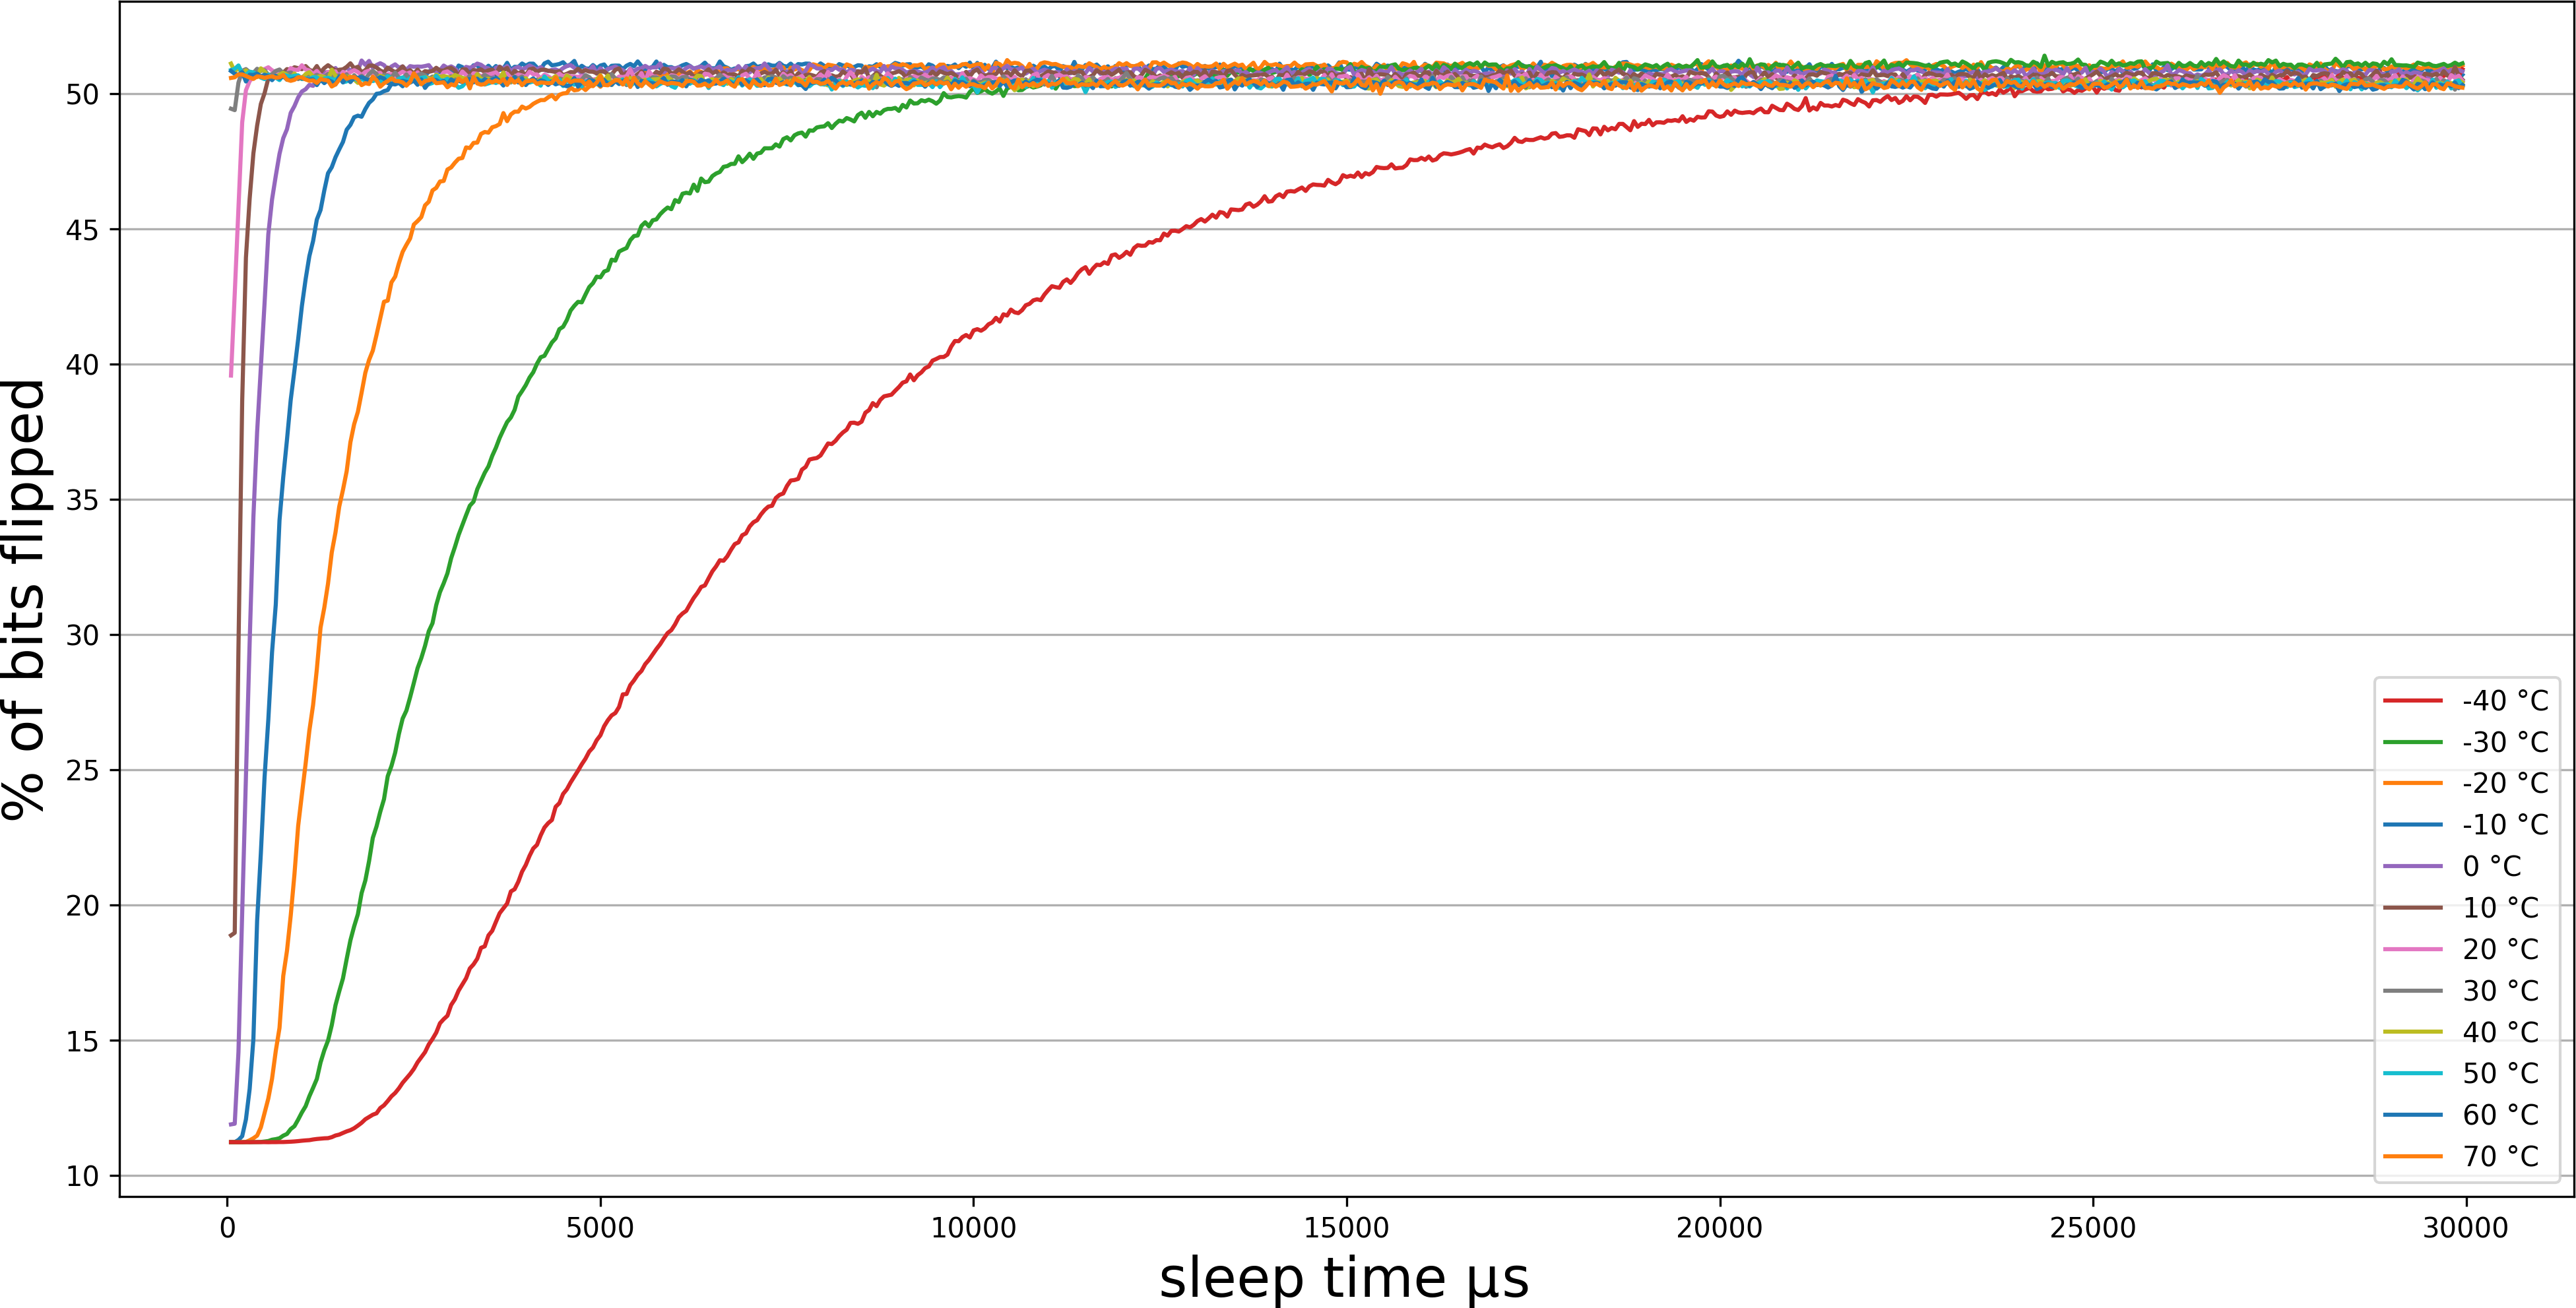
\includegraphics[width=\textwidth]{images/6_across_temps_deep_sleep.png}
    \caption{Percentage of flipped bits of MCU 6 across a range of temperatures (deep sleep method)}
    \label{fig:6_across_temps_deep_sleep}
\end{figure}
\subsection{PUF evaluation parameters}\label{sec:deepsleep_evaluation}

The \gls{puf} responses needed for the calculation of the evaluation parameters were obtained by the deep sleep power-control method. The responses were chosen to be 4~KB bit strings of the internal \gls{sram} 2 startup values. The turn off interval was set to 100~000~$\mu{}S$ since the maximal \emph{fade-out time} of memory was found to be 50~000~$\mu{}S$ plus a conservative safety margin. The reference response was calculated using a bitwise average of 1000 measured responses.

\subsubsection*{Uniformity}

Uniformity of all \glspl{mcu} across the whole range of temperatures can be seen in Table~\ref{table:uniformity_deep_sleep}. All of the results are close to the ideal value of 50 \%, though a small bias towards the `1' bit is evident (all of the results are slightly above 50~\%).

\begin{table}[ht!]
    \centering
    \begin{tabular}{c||rrrrrrrrrr}
    \toprule
    \textbf{MCU} & \textbf{-40°C} & \textbf{-30°C} & \textbf{-20°C} & \textbf{-10°C} & \textbf{0°C} & \textbf{10°C} & \textbf{20°C} & \textbf{30°C} & \textbf{50°C} & \textbf{70°C} \\
    \midrule
    1    &  51.46 &  51.33 &  51.14 &  51.01 & 50.90 & 50.75 & 50.70 & 50.67 & 50.59 & 50.54 \\
    2    &  51.55 &  51.43 &  51.25 &  51.06 & 50.94 & 50.82 & 50.67 & 50.63 & 50.56 & 50.53 \\
    3    &  51.09 &  50.97 &  50.84 &  50.72 & 50.60 & 50.47 & 50.20 & 50.18 & 50.19 & 50.22 \\
    4    &  50.66 &  50.62 &  50.49 &  50.31 & 50.22 & 50.19 & 50.17 & 50.15 & 50.08 & 50.00 \\
    5    &  50.96 &  50.83 &  50.72 &  50.58 & 50.49 & 50.38 & 50.38 & 50.33 & 50.27 & 50.22 \\
    6    &  51.19 &  51.06 &  50.90 &  50.82 & 50.71 & 50.61 & 50.46 & 50.37 & 50.30 & 50.28 \\
    7    &  51.01 &  51.02 &  50.95 &  50.85 & 50.73 & 50.68 & 50.54 & 50.49 & 50.40 & 50.37 \\
    8    &  50.95 &  50.86 &  50.73 &  50.61 & 50.47 & 50.37 & 50.23 & 50.16 & 50.01 & 49.94 \\
    9    &  51.54 &  51.36 &  51.24 &  51.14 & 51.03 & 50.91 & 50.61 & 50.53 & 50.39 & 50.40 \\
    10   &  51.37 &  51.18 &  51.03 &  50.89 & 50.78 & 50.68 & 50.50 & 50.48 & 50.36 & 50.37 \\
    11   &  51.63 &  51.54 &  51.40 &  51.28 & 51.13 & 51.06 & 50.86 & 50.86 & 50.81 & 50.81 \\
    12   &  51.56 &  51.40 &  51.23 &  51.06 & 50.93 & 50.77 & 50.57 & 50.42 & 50.27 & 50.24 \\
    13   &  50.81 &  50.71 &  50.60 &  50.55 & 50.50 & 50.48 & 50.42 & 50.34 & 50.22 & 50.15 \\
    14   &  50.26 &  50.17 &  50.11 &  50.11 & 50.03 & 50.03 & 50.02 & 50.05 & 50.14 & 50.22 \\
    15   &  51.55 &  51.45 &  51.36 &  51.32 & 51.26 & 51.16 & 51.08 & 50.98 & 50.79 & 50.64 \\
    16   &  52.43 &  52.31 &  52.24 &  52.18 & 52.07 & 51.89 & 51.81 & 51.66 & 51.26 & 50.92 \\
    \textbf{mean} &  51.25 &  51.14 &  51.01 &  50.91 & 50.80 & 50.70 & 50.58 & 50.52 & 50.42 & 50.37 \\
    \bottomrule
    \end{tabular}
    \captionsetup{justification=centering,margin=0.5cm}
    \caption{Uniformity (\%) across all MCUs and temperatures (deep sleep method, 100~mS turn off interval)}
    \label{table:uniformity_deep_sleep}
\end{table}

\subsubsection*{Reliability}

Reliability values of all \gls{mcu} in different temperatures are displayed in Table~\ref{table:reliability_deep_sleep}. The reference response was calculated at 20~°C.

The best reliability is achieved at 20~°C since the reference response was calculated at this temperature. Reliability starts to decrease in different temperatures. The decrease is proportional to the distance from the 20~°C of the reference response. However, the values are still quite close to the ideal 100 \% and they only rarely fall under 90~\% (only at -40~°C).

\begin{table}[ht!]
    \centering
    \begin{tabular}{c||rrrrrrrrrr}
    \toprule
    \textbf{MCU} & \textbf{-40°C} & \textbf{-30°C} & \textbf{-20°C} & \textbf{-10°C} & \textbf{0°C} & \textbf{10°C} & \textbf{20°C} & \textbf{30°C} & \textbf{50°C} & \textbf{70°C} \\
    \midrule
    1    &  90.36 &  91.60 &  92.80 &  93.99 & 95.03 & 95.62 & 96.13 & 95.77 & 94.47 & 92.99 \\
    2    &  91.57 &  92.53 &  93.49 &  94.43 & 95.34 & 96.04 & 96.59 & 96.16 & 94.61 & 93.04 \\
    3    &  90.19 &  91.39 &  92.55 &  93.67 & 94.76 & 95.53 & 96.15 & 95.72 & 94.17 & 92.55 \\
    4    &  90.78 &  91.97 &  93.10 &  94.10 & 95.02 & 95.60 & 96.10 & 95.74 & 94.39 & 92.90 \\
    5    &  90.72 &  91.81 &  92.93 &  94.05 & 95.10 & 95.79 & 96.28 & 95.90 & 94.57 & 93.15 \\
    6    &  90.98 &  92.23 &  93.40 &  94.44 & 95.27 & 95.80 & 96.21 & 95.91 & 94.75 & 93.44 \\
    7    &  90.29 &  91.39 &  92.55 &  93.67 & 94.73 & 95.49 & 96.03 & 95.68 & 94.24 & 92.40 \\
    8    &  90.81 &  91.91 &  93.03 &  94.10 & 95.02 & 95.67 & 96.16 & 95.72 & 94.14 & 92.26 \\
    9    &  90.91 &  91.98 &  92.96 &  93.96 & 94.92 & 95.67 & 96.28 & 95.85 & 94.13 & 92.40 \\
    10   &  90.01 &  91.21 &  92.43 &  93.68 & 94.84 & 95.61 & 96.11 & 95.73 & 94.27 & 92.54 \\
    11   &  89.87 &  91.19 &  92.56 &  93.93 & 95.07 & 95.80 & 96.24 & 95.88 & 94.60 & 93.24 \\
    12   &  90.82 &  91.96 &  93.10 &  94.20 & 95.19 & 95.85 & 96.28 & 95.93 & 94.51 & 92.83 \\
    13   &  90.83 &  91.95 &  93.12 &  94.29 & 95.34 & 96.06 & 96.34 & 95.93 & 94.41 & 92.87 \\
    14   &  90.70 &  91.91 &  93.17 &  94.34 & 95.35 & 95.94 & 96.14 & 95.70 & 94.27 & 92.67 \\
    15   &  90.21 &  91.46 &  92.66 &  93.81 & 94.91 & 95.72 & 96.01 & 95.61 & 94.15 & 92.46 \\
    16   &  89.82 &  91.02 &  92.25 &  93.52 & 94.79 & 95.83 & 96.26 & 95.64 & 93.16 & 90.24 \\
    \textbf{mean} &  90.55 &  91.72 &  92.88 &  94.01 & 95.04 & 95.75 & 96.21 & 95.80 & 94.30 & 92.62 \\
    \bottomrule
    \end{tabular}
    \captionsetup{justification=centering,margin=0.5cm}
    \caption{Reliability (\%) across all MCUs and temperatures (deep sleep method, 100~mS turn off interval)}
    \label{table:reliability_deep_sleep}
\end{table}

\subsubsection*{Uniqueness}

Uniqueness for all \glspl{mcu} across the range of different temperatures is shown in Table~\ref{table:uniqueness_deep_sleep}. The results hover just under the ideal value of 50~\% for all temperatures.

\begin{table}[ht!]
    \centering
    \begin{tabular}{cc}
        \textbf{Temperature °C} & \textbf{Uniqueness \%} \\
    \toprule
    -40  & 49.37 \\
    -30  & 49.41 \\
    -20  & 49.45 \\
    -10  & 49.49 \\
    0    & 49.51 \\
    10   & 49.56 \\
    20   & 49.61 \\
    30   & 49.63 \\
    40   & 49.66 \\
    50   & 49.68 \\
    60   & 49.70 \\
    70   & 49.73 \\
    \textbf{mean} & 49.57 \\
    \bottomrule
    \end{tabular}
    \captionsetup{justification=centering,margin=0.5cm}
    \caption{Uniqueness (\%) across all MCUs and temperatures (deep sleep method, 100~mS turn off interval)}
    \label{table:uniqueness_deep_sleep}
\end{table}

\subsection{Summary}

The presented experiments show very good results across the whole tested range of temperatures. The deep sleep functionality is available to all microcontrollers in the ESP32 family. This power-control method is therefore not restricted only to a particular subset of models. Additionally, most of the internal \gls{sram} memory (around 400~KB) is available to be used in the \gls{puf} implementation.

On the other hand, the deep sleep power-control method is especially time-consuming (in comparison to the \gls{rtc} \gls{sram} method). This is mainly due to the need to go through the whole booting process. Obtaining the response can take up to several tenths of seconds, depending on the application size and speed of the connected flash memory. Moreover, most of the device state is inevitably lost during deep sleep. The application must save all data it does not want to lose to either the FAST or SLOW \gls{rtc} \gls{sram} (the only memory regions not turned off). Although, they together only provide 16~KB of space

%--------------------------------
\section{PUF response data visualization} % TODO how to name this section?
%--------------------------------

The above-described experiments and evaluation parameters only looked at the response data globally and reduced the entire response bit string to a single number. As will become clear, it can be useful to look at the data more locally. Therefore the following visualization is presented.

The whole 4 KB \gls{puf} response is arranged bit by bit to a $256 \times 128$ grid. Black bits represent the `0' state and white bits represent the `1' state. This visualization of 4 responses from different \glspl{mcu} can be seen in Figure~\ref{fig:puf_response_visualization}. The first two responses were obtained using the deep sleep method and the last two using the \gls{rtc} \gls{sram} method.

The response from \gls{mcu} 1 (\ref{fig:mcu_1}) looks as expected, the bits are arranged in a random-looking pattern\footnote{This, of course, is not proof that the bits really are random}. However, the other responses show strange stripes. Every 32 bits the startup bias of memory cells towards a certain state flips. This results in this stripe-looking pattern. The previous experiments did not reveal this behavior (mainly uniformity), as the overall number of  `0' and `1' bits stays the same globally.

Both power-control methods produce the same result. Additionally, some of the \glspl{mcu} do not exhibit this behavior at all (\ref{fig:mcu_1}), some of them show only a slight `stripe-like' bias (\ref{fig:mcu_13},~\ref{fig:mcu_3}), and some are affected in a lot (\ref{fig:mcu_11}).

\begin{figure}[ht!]
        \centering
        \captionsetup{justification=centering,margin=0.5cm}
        \begin{subfigure}[b]{0.475\textwidth}
            \centering
            
\includegraphics[width=\textwidth]{images/1_response_sleep.png}
            \caption{MCU 1 (deep sleep method)}    
            \label{fig:mcu_1}
        \end{subfigure}
        \hfill
        \begin{subfigure}[b]{0.475\textwidth}  
            \centering 
            
\includegraphics[width=\textwidth]{images/13_response_sleep.png}
            \caption{MCU 13 (deep sleep method)}    
            \label{fig:mcu_13}
        \end{subfigure}
        \vskip 1.75mm
        \begin{subfigure}[b]{0.475\textwidth}   
            \centering 
            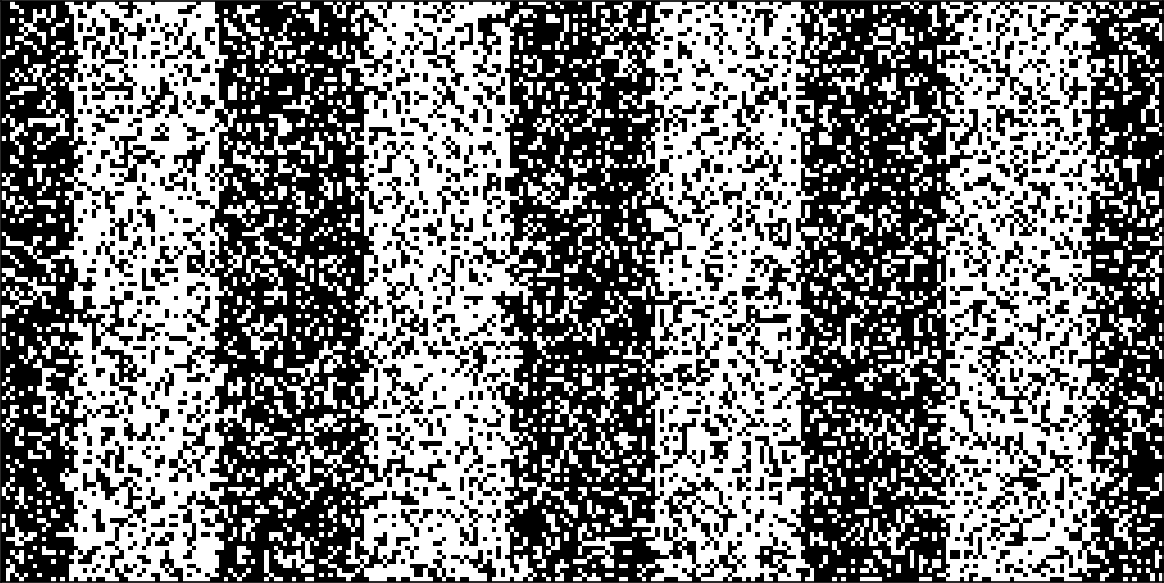
\includegraphics[width=\textwidth]{images/11_response_rtc.png}
            \caption{MCU 11 (RTC SRAM method)}    
            \label{fig:mcu_11}
        \end{subfigure}
        \hfill
        \begin{subfigure}[b]{0.475\textwidth}   
            \centering 
            
\includegraphics[width=\textwidth]{images/3_response_rtc.png}
            \caption{MCU 3 (RTC SRAM method)}    
            \label{fig:mcu_3}
        \end{subfigure}
        \caption{Visualization of PUF responses from different MCUs} 
        \label{fig:puf_response_visualization}
\end{figure}

One edge case was also revealed. \Gls{mcu} 16 exhibited different behavior from all of the other \glspl{mcu}. Its `stripes' are 256 bits wide. In order to visualize this, the grid was reshaped into a $512 \times 64$ configuration which is shown in Figure~\ref{fig:16_response_sleep}.

However, only the \gls{rtc} \gls{sram} method shows this wide stripe behavior. This is probably not due to the different power-state control of memory, but rather because a different memory region is used for the response extraction.

\begin{figure}[ht!]
    \centering
    \captionsetup{justification=centering,margin=0.5cm}
    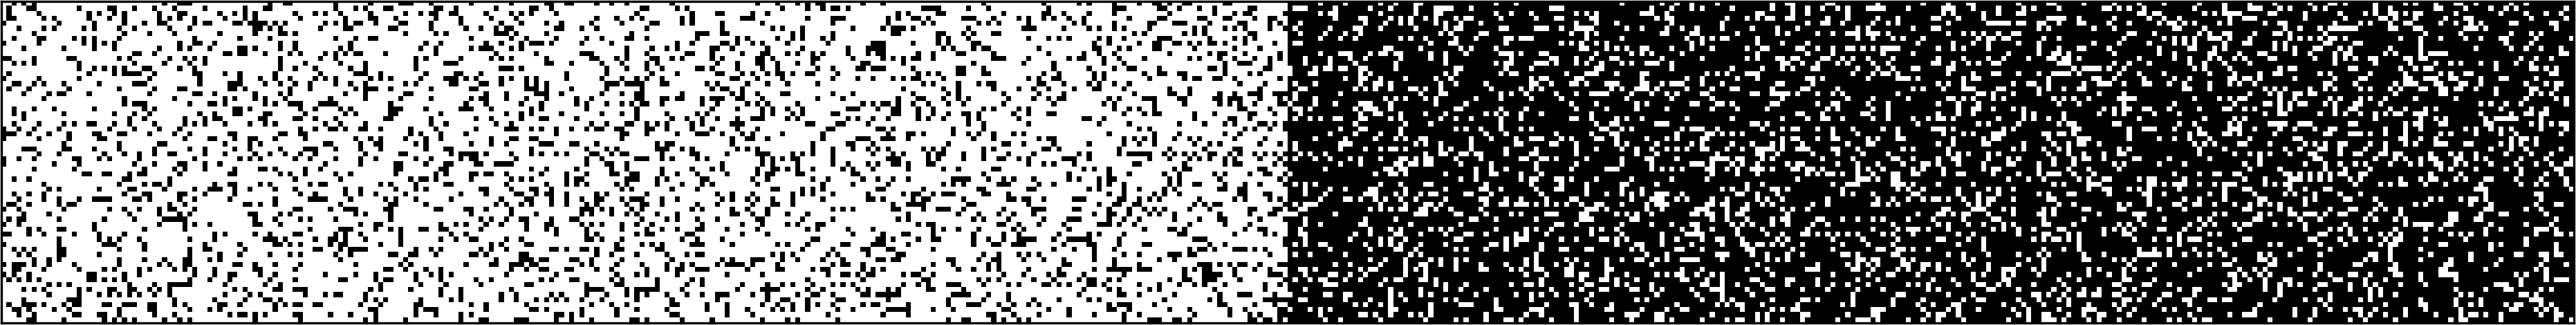
\includegraphics[width=\textwidth]{images/16_response_sleep.png}
    \caption{Visualization of PUF response from MCU 16 (RTC SRAM method).}
    \label{fig:16_response_sleep}
\end{figure}

This behavior is most likely caused by the internal design of the \gls{sram} circuit and there is probably no way to prevent it. This explanation unfortunately cannot be confirmed as the ESP32 chip schematics are not available. It is, however, clear that the entropy of the resulting \gls{puf} response is reduced because of this behavior.

In order to improve the statistical properties of the \gls{puf} responses, a cryptographic hash function can be applied before using it. This is especially important if the \gls{puf} is used to generate a cryptographic key.~\cite{Sven2015},~\cite{Dodis2008}

